% \section{Experiment: Scrabble String Problem}

\begin{frame}{Problem Definition}
\textbf{phenotype:} 100-letter string with characters a,b,\dots,z,``~''
\vspace{2ex}
\pause

\textbf{fitness:} count of characters contained in valid Scrabble words
\begin{itemize}
\item best fitness = long valid words
\end{itemize}

\vspace{2ex}
\pause

\textbf{rugged fitness landscape:}
short words are difficult to combine without becoming invalid

\end{frame}

\begin{frame}{Denoiser Genotype-Phenotype Map Implementation}

\begin{figure}
  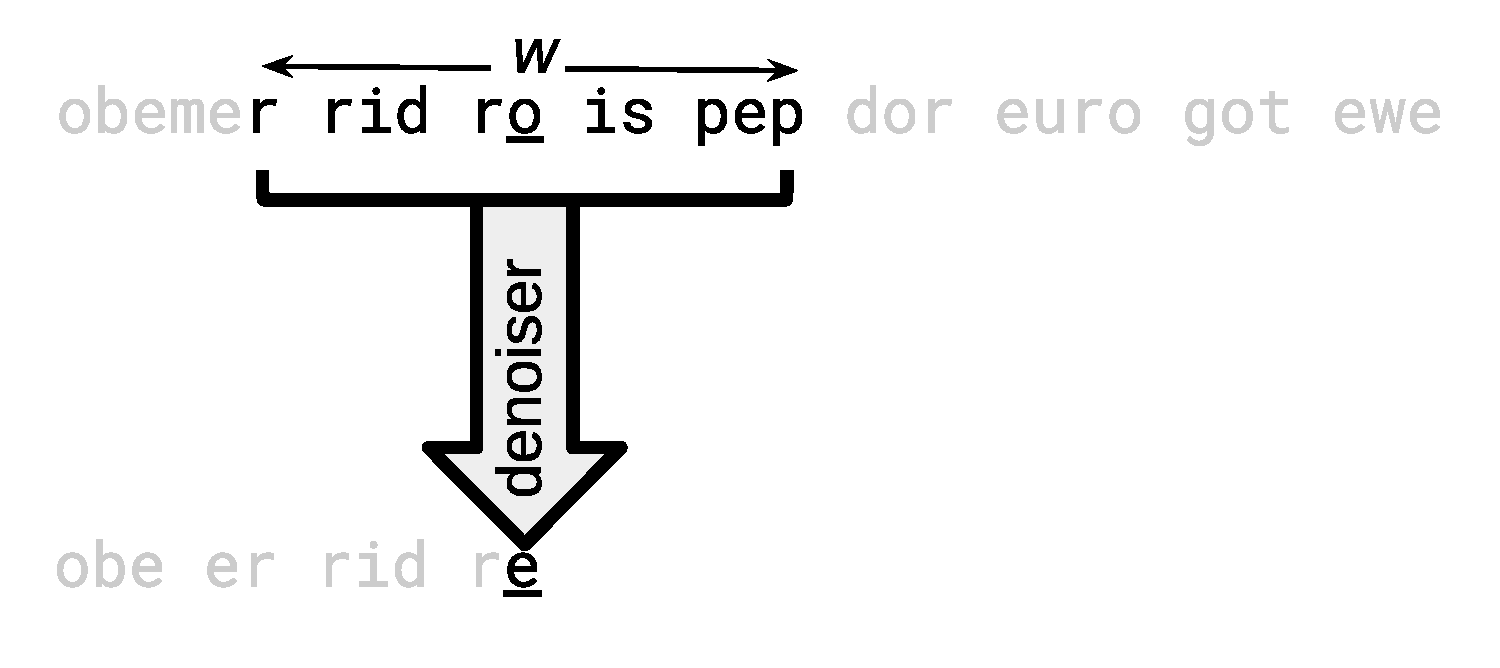
\includegraphics[width=\textwidth]{img/scrabble_denoiser_in_action}
  \caption{
    Illustration of denoising autoencoder in action in the Scrabble domain.
  }\label{fig:scrabble_denoiser_in_action}
\end{figure}


\end{frame}

\begin{frame}{Training Pipeline}

\centering \Large

\textcolor{h2}{$\downarrow$ evolve word strings with direct encoding $\downarrow$}

\dots\texttt{ns fed oxo sob }\dots

\pause

\textcolor{h2}{$\downarrow$ corrupt letter (sometimes) $\downarrow$}

\dots\texttt{ns fed \fbox{p}xo sob }\dots

\pause

\textcolor{h2}{$\downarrow$ autoencoder guesses original letter $\downarrow$}

\texttt{\fbox{o}}

\pause

\textcolor{h2}{$\downarrow$ check guess $\downarrow$}

if wrong, adjust autoencoder

\end{frame}

\begin{frame}{Result: Viability under Mutation}

\begin{figure}
  \includegraphics[width=0.8\linewidth]<1>{img/results/scrabble_fit_diff_vs_step-1}
  \includegraphics[width=0.8\linewidth]<2>{img/results/scrabble_fit_diff_vs_step-2}
  \caption{
    Fitness loss by mutational step in the Scrabble string domain.
    Bootstrapped 95\% confidence intervals are shaded along each curve.
    }\label{fig:scrabble_fit_diff_vs_step}
\end{figure}


\end{frame}

\begin{frame}{Result: Novelty under Mutation}

\begin{figure}
  \includegraphics[width=0.85\linewidth]<1>{img/results/scrabble_dist_vs_step-1}
  \includegraphics[width=0.85\linewidth]<2>{img/results/scrabble_dist_vs_step-2}
  \caption{
    Phenotypic divergence by mutational step in the Scrabble string domain.
    Bootstrapped 95\% confidence intervals are shaded along each curve.
  }\label{fig:scrabble_dist_vs_step}
\end{figure}


\end{frame}

\begin{frame}{Scrabble Result: Evolvability Signature}

\begin{figure}
  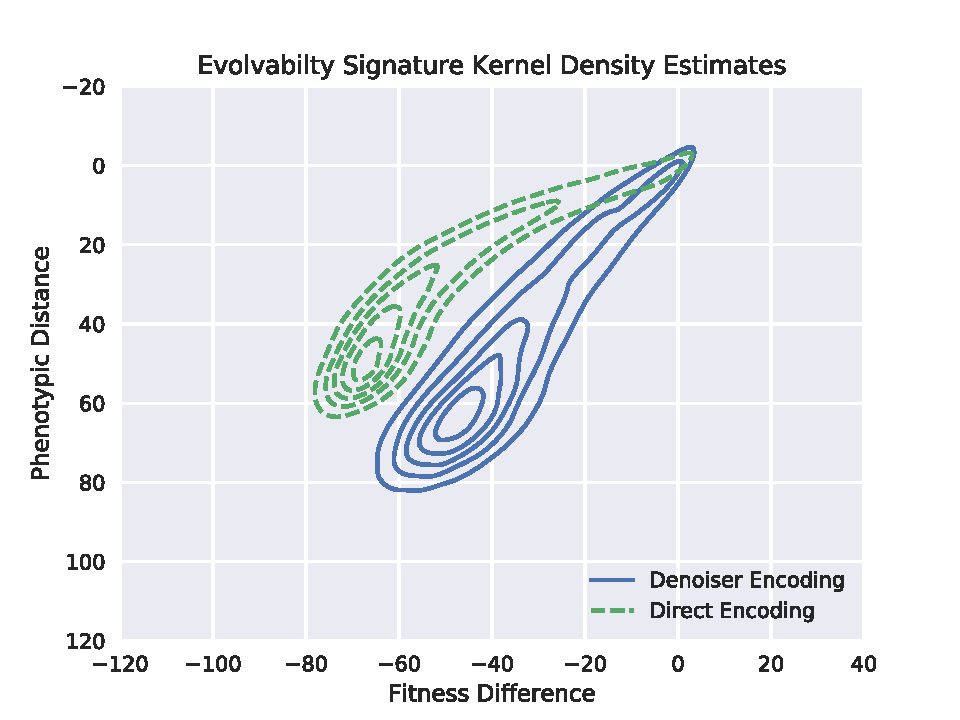
\includegraphics[width=0.8\linewidth]{img/results/scrabble_es_kde}
  \caption{
    Gaussian kernel density estimates for evolvability signatures of direct and indirect encodings in Scrabble string domain \cite{tarapore2015evolvability}.
  }\label{fig:scrabble_es_kde}
\end{figure}


\end{frame}
